\documentclass[1p]{elsarticle_modified}
%\bibliographystyle{elsarticle-num}

%\usepackage[colorlinks]{hyperref}
%\usepackage{abbrmath_seonhwa} %\Abb, \Ascr, \Acal ,\Abf, \Afrak
\usepackage{amsfonts}
\usepackage{amssymb}
\usepackage{amsmath}
\usepackage{amsthm}
\usepackage{scalefnt}
\usepackage{amsbsy}
\usepackage{kotex}
\usepackage{caption}
\usepackage{subfig}
\usepackage{color}
\usepackage{graphicx}
\usepackage{xcolor} %% white, black, red, green, blue, cyan, magenta, yellow
\usepackage{float}
\usepackage{setspace}
\usepackage{hyperref}

\usepackage{tikz}
\usetikzlibrary{arrows}

\usepackage{multirow}
\usepackage{array} % fixed length table
\usepackage{hhline}

%%%%%%%%%%%%%%%%%%%%%
\makeatletter
\renewcommand*\env@matrix[1][\arraystretch]{%
	\edef\arraystretch{#1}%
	\hskip -\arraycolsep
	\let\@ifnextchar\new@ifnextchar
	\array{*\c@MaxMatrixCols c}}
\makeatother %https://tex.stackexchange.com/questions/14071/how-can-i-increase-the-line-spacing-in-a-matrix
%%%%%%%%%%%%%%%

\usepackage[normalem]{ulem}

\newcommand{\msout}[1]{\ifmmode\text{\sout{\ensuremath{#1}}}\else\sout{#1}\fi}
%SOURCE: \msout is \stkout macro in https://tex.stackexchange.com/questions/20609/strikeout-in-math-mode

\newcommand{\cancel}[1]{
	\ifmmode
	{\color{red}\msout{#1}}
	\else
	{\color{red}\sout{#1}}
	\fi
}

\newcommand{\add}[1]{
	{\color{blue}\uwave{#1}}
}

\newcommand{\replace}[2]{
	\ifmmode
	{\color{red}\msout{#1}}{\color{blue}\uwave{#2}}
	\else
	{\color{red}\sout{#1}}{\color{blue}\uwave{#2}}
	\fi
}

\newcommand{\Sol}{\mathcal{S}} %segment
\newcommand{\D}{D} %diagram
\newcommand{\A}{\mathcal{A}} %arc


%%%%%%%%%%%%%%%%%%%%%%%%%%%%%5 test

\def\sl{\operatorname{\textup{SL}}(2,\Cbb)}
\def\psl{\operatorname{\textup{PSL}}(2,\Cbb)}
\def\quan{\mkern 1mu \triangleright \mkern 1mu}

\theoremstyle{definition}
\newtheorem{thm}{Theorem}[section]
\newtheorem{prop}[thm]{Proposition}
\newtheorem{lem}[thm]{Lemma}
\newtheorem{ques}[thm]{Question}
\newtheorem{cor}[thm]{Corollary}
\newtheorem{defn}[thm]{Definition}
\newtheorem{exam}[thm]{Example}
\newtheorem{rmk}[thm]{Remark}
\newtheorem{alg}[thm]{Algorithm}

\newcommand{\I}{\sqrt{-1}}
\begin{document}

%\begin{frontmatter}
%
%\title{Boundary parabolic representations of knots up to 8 crossings}
%
%%% Group authors per affiliation:
%\author{Yunhi Cho} 
%\address{Department of Mathematics, University of Seoul, Seoul, Korea}
%\ead{yhcho@uos.ac.kr}
%
%
%\author{Seonhwa Kim} %\fnref{s_kim}}
%\address{Center for Geometry and Physics, Institute for Basic Science, Pohang, 37673, Korea}
%\ead{ryeona17@ibs.re.kr}
%
%\author{Hyuk Kim}
%\address{Department of Mathematical Sciences, Seoul National University, Seoul 08826, Korea}
%\ead{hyukkim@snu.ac.kr}
%
%\author{Seokbeom Yoon}
%\address{Department of Mathematical Sciences, Seoul National University, Seoul, 08826,  Korea}
%\ead{sbyoon15@snu.ac.kr}
%
%\begin{abstract}
%We find all boundary parabolic representation of knots up to 8 crossings.
%
%\end{abstract}
%\begin{keyword}
%    \MSC[2010] 57M25 
%\end{keyword}
%
%\end{frontmatter}

%\linenumbers
%\tableofcontents
%
\newcommand\colored[1]{\textcolor{white}{\rule[-0.35ex]{0.8em}{1.4ex}}\kern-0.8em\color{red} #1}%
%\newcommand\colored[1]{\textcolor{white}{ #1}\kern-2.17ex	\textcolor{white}{ #1}\kern-1.81ex	\textcolor{white}{ #1}\kern-2.15ex\color{red}#1	}

{\Large $\underline{11a_{72}~(K11a_{72})}$}

\setlength{\tabcolsep}{10pt}
\renewcommand{\arraystretch}{1.6}
\vspace{1cm}\begin{tabular}{m{100pt}>{\centering\arraybackslash}m{274pt}}
\multirow{5}{120pt}{
	\centering
	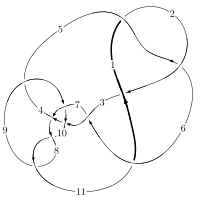
\includegraphics[width=112pt]{../../../GIT/diagram.site/Diagrams/png/321_11a_72.png}\\
\ \ \ A knot diagram\footnotemark}&
\allowdisplaybreaks
\textbf{Linearized knot diagam} \\
\cline{2-2}
 &
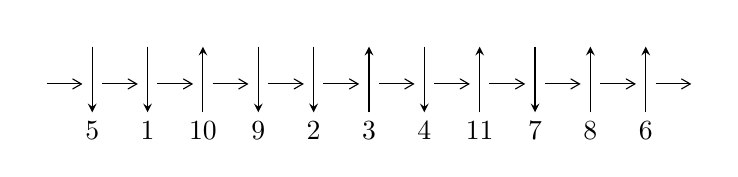
\begin{tikzpicture}[x=20pt, y=17pt]
	% nodes
	\node (C0) at (0, 0) {};
	\node (C1) at (1, 0) {};
	\node (C1U) at (1, +1) {};
	\node (C1D) at (1, -1) {5};

	\node (C2) at (2, 0) {};
	\node (C2U) at (2, +1) {};
	\node (C2D) at (2, -1) {1};

	\node (C3) at (3, 0) {};
	\node (C3U) at (3, +1) {};
	\node (C3D) at (3, -1) {10};

	\node (C4) at (4, 0) {};
	\node (C4U) at (4, +1) {};
	\node (C4D) at (4, -1) {9};

	\node (C5) at (5, 0) {};
	\node (C5U) at (5, +1) {};
	\node (C5D) at (5, -1) {2};

	\node (C6) at (6, 0) {};
	\node (C6U) at (6, +1) {};
	\node (C6D) at (6, -1) {3};

	\node (C7) at (7, 0) {};
	\node (C7U) at (7, +1) {};
	\node (C7D) at (7, -1) {4};

	\node (C8) at (8, 0) {};
	\node (C8U) at (8, +1) {};
	\node (C8D) at (8, -1) {11};

	\node (C9) at (9, 0) {};
	\node (C9U) at (9, +1) {};
	\node (C9D) at (9, -1) {7};

	\node (C10) at (10, 0) {};
	\node (C10U) at (10, +1) {};
	\node (C10D) at (10, -1) {8};

	\node (C11) at (11, 0) {};
	\node (C11U) at (11, +1) {};
	\node (C11D) at (11, -1) {6};
	\node (C12) at (12, 0) {};

	% arrows
	\draw[->,>={angle 60}]
	(C0) edge (C1) (C1) edge (C2) (C2) edge (C3) (C3) edge (C4) (C4) edge (C5) (C5) edge (C6) (C6) edge (C7) (C7) edge (C8) (C8) edge (C9) (C9) edge (C10) (C10) edge (C11) (C11) edge (C12) ;	\draw[->,>=stealth]
	(C1U) edge (C1D) (C2U) edge (C2D) (C3D) edge (C3U) (C4U) edge (C4D) (C5U) edge (C5D) (C6D) edge (C6U) (C7U) edge (C7D) (C8D) edge (C8U) (C9U) edge (C9D) (C10D) edge (C10U) (C11D) edge (C11U) ;
	\end{tikzpicture} \\
\hhline{~~} \\& 
\textbf{Solving Sequence} \\ \cline{2-2} 
 &
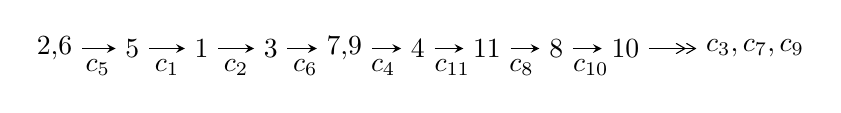
\begin{tikzpicture}[x=25pt, y=7pt]
	% node
	\node (A0) at (-1/8, 0) {2,6};
	\node (A1) at (1, 0) {5};
	\node (A2) at (2, 0) {1};
	\node (A3) at (3, 0) {3};
	\node (A4) at (65/16, 0) {7,9};
	\node (A5) at (41/8, 0) {4};
	\node (A6) at (49/8, 0) {11};
	\node (A7) at (57/8, 0) {8};
	\node (A8) at (65/8, 0) {10};
	\node (C1) at (1/2, -1) {$c_{5}$};
	\node (C2) at (3/2, -1) {$c_{1}$};
	\node (C3) at (5/2, -1) {$c_{2}$};
	\node (C4) at (7/2, -1) {$c_{6}$};
	\node (C5) at (37/8, -1) {$c_{4}$};
	\node (C6) at (45/8, -1) {$c_{11}$};
	\node (C7) at (53/8, -1) {$c_{8}$};
	\node (C8) at (61/8, -1) {$c_{10}$};
	\node (A9) at (10, 0) {$c_{3},c_{7},c_{9}$};

	% edge
	\draw[->,>=stealth]	
	(A0) edge (A1) (A1) edge (A2) (A2) edge (A3) (A3) edge (A4) (A4) edge (A5) (A5) edge (A6) (A6) edge (A7) (A7) edge (A8) ;
	\draw[->>,>={angle 60}]	
	(A8) edge (A9);
\end{tikzpicture} \\ 

\end{tabular} \\

\footnotetext{
The image of knot diagram is generated by the software ``\textbf{Draw programme}" developed by Andrew Bartholomew(\url{http://www.layer8.co.uk/maths/draw/index.htm\#Running-draw}), where we modified some parts for our purpose(\url{https://github.com/CATsTAILs/LinksPainter}).
}\phantom \\ \newline 
\centering \textbf{Ideals for irreducible components\footnotemark of $X_{\text{par}}$} 
 
\begin{align*}
I^u_{1}&=\langle 
9.34803\times10^{24} u^{76}-2.11084\times10^{24} u^{75}+\cdots+9.10663\times10^{24} b+2.06273\times10^{24},\\
\phantom{I^u_{1}}&\phantom{= \langle  }2.74420\times10^{25} u^{76}-4.20119\times10^{25} u^{75}+\cdots+9.10663\times10^{24} a+1.31742\times10^{25},\;u^{77}-2 u^{76}+\cdots- u-1\rangle \\
I^u_{2}&=\langle 
b+1,\;a-2,\;u+1\rangle \\
\\
\end{align*}
\raggedright * 2 irreducible components of $\dim_{\mathbb{C}}=0$, with total 78 representations.\\
\footnotetext{All coefficients of polynomials are rational numbers. But the coefficients are sometimes approximated in decimal forms when there is not enough margin.}
\newpage
\renewcommand{\arraystretch}{1}
\centering \section*{I. $I^u_{1}= \langle 9.35\times10^{24} u^{76}-2.11\times10^{24} u^{75}+\cdots+9.11\times10^{24} b+2.06\times10^{24},\;2.74\times10^{25} u^{76}-4.20\times10^{25} u^{75}+\cdots+9.11\times10^{24} a+1.32\times10^{25},\;u^{77}-2 u^{76}+\cdots- u-1 \rangle$}
\flushleft \textbf{(i) Arc colorings}\\
\begin{tabular}{m{7pt} m{180pt} m{7pt} m{180pt} }
\flushright $a_{2}=$&$\begin{pmatrix}0\\u\end{pmatrix}$ \\
\flushright $a_{6}=$&$\begin{pmatrix}1\\0\end{pmatrix}$ \\
\flushright $a_{5}=$&$\begin{pmatrix}1\\- u^2\end{pmatrix}$ \\
\flushright $a_{1}=$&$\begin{pmatrix}u\\- u^3+u\end{pmatrix}$ \\
\flushright $a_{3}=$&$\begin{pmatrix}- u^3\\u^5- u^3+u\end{pmatrix}$ \\
\flushright $a_{7}=$&$\begin{pmatrix}u^8- u^6+u^4+1\\- u^{10}+2 u^8-3 u^6+2 u^4- u^2\end{pmatrix}$ \\
\flushright $a_{9}=$&$\begin{pmatrix}-3.01341 u^{76}+4.61333 u^{75}+\cdots-6.55819 u-1.44666\\-1.02651 u^{76}+0.231791 u^{75}+\cdots+2.18024 u-0.226508\end{pmatrix}$ \\
\flushright $a_{4}=$&$\begin{pmatrix}-4.68917 u^{76}+6.28660 u^{75}+\cdots-16.1580 u-3.80329\\0.0425498 u^{76}-0.839980 u^{75}+\cdots+2.36327 u+0.839980\end{pmatrix}$ \\
\flushright $a_{11}=$&$\begin{pmatrix}u^3\\- u^3+u\end{pmatrix}$ \\
\flushright $a_{8}=$&$\begin{pmatrix}-2.84647 u^{76}+4.44668 u^{75}+\cdots-6.17515 u-1.26334\\-0.993730 u^{76}+0.182343 u^{75}+\cdots+1.42940 u-0.193730\end{pmatrix}$ \\
\flushright $a_{10}=$&$\begin{pmatrix}-2.78104 u^{76}+4.37995 u^{75}+\cdots-7.68244 u-1.12997\\-1.05786 u^{76}+0.320078 u^{75}+\cdots+2.03322 u-0.257856\end{pmatrix}$\\ \flushright $a_{10}=$&$\begin{pmatrix}-2.78104 u^{76}+4.37995 u^{75}+\cdots-7.68244 u-1.12997\\-1.05786 u^{76}+0.320078 u^{75}+\cdots+2.03322 u-0.257856\end{pmatrix}$\\&\end{tabular}
\flushleft \textbf{(ii) Obstruction class $= -1$}\\~\\
\flushleft \textbf{(iii) Cusp Shapes $= -\frac{98621680931509431399030560}{4553313053666260493091767} u^{76}+\frac{105996530335693508948090410}{4553313053666260493091767} u^{75}+\cdots-\frac{186890667880794717580337970}{4553313053666260493091767} u-\frac{85143874290832413279068140}{4553313053666260493091767}$}\\~\\
\newpage\renewcommand{\arraystretch}{1}
\flushleft \textbf{(iv) u-Polynomials at the component}\newline \\
\begin{tabular}{m{50pt}|m{274pt}}
Crossings & \hspace{64pt}u-Polynomials at each crossing \\
\hline $$\begin{aligned}c_{1},c_{5}\end{aligned}$$&$\begin{aligned}
&u^{77}+2 u^{76}+\cdots- u+1
\end{aligned}$\\
\hline $$\begin{aligned}c_{2}\end{aligned}$$&$\begin{aligned}
&u^{77}+36 u^{76}+\cdots- u+1
\end{aligned}$\\
\hline $$\begin{aligned}c_{3}\end{aligned}$$&$\begin{aligned}
&u^{77}-4 u^{76}+\cdots-1931 u+431
\end{aligned}$\\
\hline $$\begin{aligned}c_{4}\end{aligned}$$&$\begin{aligned}
&u^{77}-2 u^{76}+\cdots+22949 u+1393
\end{aligned}$\\
\hline $$\begin{aligned}c_{6}\end{aligned}$$&$\begin{aligned}
&u^{77}-22 u^{75}+\cdots-44155 u+8353
\end{aligned}$\\
\hline $$\begin{aligned}c_{7}\end{aligned}$$&$\begin{aligned}
&u^{77}+4 u^{76}+\cdots+u+1
\end{aligned}$\\
\hline $$\begin{aligned}c_{8},c_{10}\end{aligned}$$&$\begin{aligned}
&u^{77}+2 u^{76}+\cdots- u+1
\end{aligned}$\\
\hline $$\begin{aligned}c_{9}\end{aligned}$$&$\begin{aligned}
&u^{77}-13 u^{76}+\cdots+2 u+2
\end{aligned}$\\
\hline $$\begin{aligned}c_{11}\end{aligned}$$&$\begin{aligned}
&u^{77}+3 u^{76}+\cdots+523 u^2+32
\end{aligned}$\\
\hline
\end{tabular}\\~\\
\newpage\renewcommand{\arraystretch}{1}
\flushleft \textbf{(v) Riley Polynomials at the component}\newline \\
\begin{tabular}{m{50pt}|m{274pt}}
Crossings & \hspace{64pt}Riley Polynomials at each crossing \\
\hline $$\begin{aligned}c_{1},c_{5}\end{aligned}$$&$\begin{aligned}
&y^{77}-36 y^{76}+\cdots- y-1
\end{aligned}$\\
\hline $$\begin{aligned}c_{2}\end{aligned}$$&$\begin{aligned}
&y^{77}+12 y^{76}+\cdots-69 y-1
\end{aligned}$\\
\hline $$\begin{aligned}c_{3}\end{aligned}$$&$\begin{aligned}
&y^{77}-92 y^{76}+\cdots+8518895 y-185761
\end{aligned}$\\
\hline $$\begin{aligned}c_{4}\end{aligned}$$&$\begin{aligned}
&y^{77}-48 y^{76}+\cdots+99292559 y-1940449
\end{aligned}$\\
\hline $$\begin{aligned}c_{6}\end{aligned}$$&$\begin{aligned}
&y^{77}-44 y^{76}+\cdots+683599815 y-69772609
\end{aligned}$\\
\hline $$\begin{aligned}c_{7}\end{aligned}$$&$\begin{aligned}
&y^{77}+12 y^{76}+\cdots- y-1
\end{aligned}$\\
\hline $$\begin{aligned}c_{8},c_{10}\end{aligned}$$&$\begin{aligned}
&y^{77}-56 y^{76}+\cdots-21 y-1
\end{aligned}$\\
\hline $$\begin{aligned}c_{9}\end{aligned}$$&$\begin{aligned}
&y^{77}+9 y^{76}+\cdots-40 y-4
\end{aligned}$\\
\hline $$\begin{aligned}c_{11}\end{aligned}$$&$\begin{aligned}
&y^{77}+9 y^{76}+\cdots-33472 y-1024
\end{aligned}$\\
\hline
\end{tabular}\\~\\
\newpage\flushleft \textbf{(vi) Complex Volumes and Cusp Shapes}
$$\begin{array}{c|c|c}  
\text{Solutions to }I^u_{1}& \I (\text{vol} + \sqrt{-1}CS) & \text{Cusp shape}\\
 \hline 
\begin{aligned}
u &= -0.633423 + 0.760124 I \\
a &= -0.611333 - 0.236752 I \\
b &= -0.164228 + 0.298926 I\end{aligned}
 & \phantom{-}7.04838 + 0.24930 I & \phantom{-0.000000 } 0 \\ \hline\begin{aligned}
u &= -0.633423 - 0.760124 I \\
a &= -0.611333 + 0.236752 I \\
b &= -0.164228 - 0.298926 I\end{aligned}
 & \phantom{-}7.04838 - 0.24930 I & \phantom{-0.000000 } 0 \\ \hline\begin{aligned}
u &= -0.976497 + 0.154539 I \\
a &= \phantom{-}1.94444 + 0.74223 I \\
b &= -1.75615 + 0.52296 I\end{aligned}
 & \phantom{-}1.58545 - 1.56270 I & \phantom{-0.000000 } 0 \\ \hline\begin{aligned}
u &= -0.976497 - 0.154539 I \\
a &= \phantom{-}1.94444 - 0.74223 I \\
b &= -1.75615 - 0.52296 I\end{aligned}
 & \phantom{-}1.58545 + 1.56270 I & \phantom{-0.000000 } 0 \\ \hline\begin{aligned}
u &= \phantom{-}0.980965 + 0.263279 I \\
a &= -5.16701 + 1.31783 I \\
b &= \phantom{-}2.20127 + 1.66225 I\end{aligned}
 & -0.098989 - 0.629989 I & \phantom{-0.000000 } 0 \\ \hline\begin{aligned}
u &= \phantom{-}0.980965 - 0.263279 I \\
a &= -5.16701 - 1.31783 I \\
b &= \phantom{-}2.20127 - 1.66225 I\end{aligned}
 & -0.098989 + 0.629989 I & \phantom{-0.000000 } 0 \\ \hline\begin{aligned}
u &= \phantom{-}0.602244 + 0.740774 I \\
a &= \phantom{-}0.487640 - 0.874753 I \\
b &= \phantom{-}0.138617 + 0.833361 I\end{aligned}
 & \phantom{-}7.76295 - 8.98786 I & \phantom{-}5.03981 + 6.60179 I \\ \hline\begin{aligned}
u &= \phantom{-}0.602244 - 0.740774 I \\
a &= \phantom{-}0.487640 + 0.874753 I \\
b &= \phantom{-}0.138617 - 0.833361 I\end{aligned}
 & \phantom{-}7.76295 + 8.98786 I & \phantom{-}5.03981 - 6.60179 I \\ \hline\begin{aligned}
u &= \phantom{-}1.001230 + 0.352341 I \\
a &= \phantom{-}2.57836 + 0.25405 I \\
b &= -0.34696 - 2.11296 I\end{aligned}
 & -0.63003 - 1.40723 I & \phantom{-0.000000 } 0 \\ \hline\begin{aligned}
u &= \phantom{-}1.001230 - 0.352341 I \\
a &= \phantom{-}2.57836 - 0.25405 I \\
b &= -0.34696 + 2.11296 I\end{aligned}
 & -0.63003 + 1.40723 I & \phantom{-0.000000 } 0\\
 \hline 
 \end{array}$$\newpage$$\begin{array}{c|c|c}  
\text{Solutions to }I^u_{1}& \I (\text{vol} + \sqrt{-1}CS) & \text{Cusp shape}\\
 \hline 
\begin{aligned}
u &= -0.986878 + 0.427459 I \\
a &= -1.09537 + 1.40681 I \\
b &= -0.15416 - 2.04505 I\end{aligned}
 & \phantom{-}0.14403 + 4.20779 I & \phantom{-0.000000 } 0 \\ \hline\begin{aligned}
u &= -0.986878 - 0.427459 I \\
a &= -1.09537 - 1.40681 I \\
b &= -0.15416 + 2.04505 I\end{aligned}
 & \phantom{-}0.14403 - 4.20779 I & \phantom{-0.000000 } 0 \\ \hline\begin{aligned}
u &= -0.857333 + 0.345143 I \\
a &= \phantom{-}1.55446 + 0.57642 I \\
b &= -1.251310 - 0.537113 I\end{aligned}
 & \phantom{-}2.25018 + 1.60092 I & \phantom{-}4.93810 - 3.13192 I \\ \hline\begin{aligned}
u &= -0.857333 - 0.345143 I \\
a &= \phantom{-}1.55446 - 0.57642 I \\
b &= -1.251310 + 0.537113 I\end{aligned}
 & \phantom{-}2.25018 - 1.60092 I & \phantom{-}4.93810 + 3.13192 I \\ \hline\begin{aligned}
u &= -0.390473 + 0.833868 I \\
a &= -0.426341 + 0.195318 I \\
b &= -0.962283 - 0.945326 I\end{aligned}
 & \phantom{-}5.65147 - 3.46025 I & \phantom{-}8.06773 + 5.13180 I \\ \hline\begin{aligned}
u &= -0.390473 - 0.833868 I \\
a &= -0.426341 - 0.195318 I \\
b &= -0.962283 + 0.945326 I\end{aligned}
 & \phantom{-}5.65147 + 3.46025 I & \phantom{-}8.06773 - 5.13180 I \\ \hline\begin{aligned}
u &= \phantom{-}1.057940 + 0.262256 I \\
a &= \phantom{-}0.163573 + 0.640731 I \\
b &= \phantom{-}0.273950 - 0.088341 I\end{aligned}
 & -2.24047 - 0.49207 I & \phantom{-0.000000 } 0 \\ \hline\begin{aligned}
u &= \phantom{-}1.057940 - 0.262256 I \\
a &= \phantom{-}0.163573 - 0.640731 I \\
b &= \phantom{-}0.273950 + 0.088341 I\end{aligned}
 & -2.24047 + 0.49207 I & \phantom{-0.000000 } 0 \\ \hline\begin{aligned}
u &= -1.081720 + 0.191062 I \\
a &= \phantom{-}1.184630 + 0.277945 I \\
b &= -0.759225 + 0.986911 I\end{aligned}
 & -2.82137 - 3.73074 I & \phantom{-0.000000 } 0 \\ \hline\begin{aligned}
u &= -1.081720 - 0.191062 I \\
a &= \phantom{-}1.184630 - 0.277945 I \\
b &= -0.759225 - 0.986911 I\end{aligned}
 & -2.82137 + 3.73074 I & \phantom{-0.000000 } 0\\
 \hline 
 \end{array}$$\newpage$$\begin{array}{c|c|c}  
\text{Solutions to }I^u_{1}& \I (\text{vol} + \sqrt{-1}CS) & \text{Cusp shape}\\
 \hline 
\begin{aligned}
u &= \phantom{-}0.387547 + 0.806255 I \\
a &= \phantom{-}0.563280 + 0.658078 I \\
b &= \phantom{-}1.72067 - 1.45490 I\end{aligned}
 & \phantom{-}6.58364 + 11.91200 I & \phantom{-}3.84588 - 6.37900 I \\ \hline\begin{aligned}
u &= \phantom{-}0.387547 - 0.806255 I \\
a &= \phantom{-}0.563280 - 0.658078 I \\
b &= \phantom{-}1.72067 + 1.45490 I\end{aligned}
 & \phantom{-}6.58364 - 11.91200 I & \phantom{-}3.84588 + 6.37900 I \\ \hline\begin{aligned}
u &= \phantom{-}0.541842 + 0.673198 I \\
a &= \phantom{-}0.09318 + 1.41546 I \\
b &= \phantom{-}0.631068 - 0.608537 I\end{aligned}
 & \phantom{-}2.59107 - 3.68436 I & \phantom{-}3.37129 + 6.54731 I \\ \hline\begin{aligned}
u &= \phantom{-}0.541842 - 0.673198 I \\
a &= \phantom{-}0.09318 - 1.41546 I \\
b &= \phantom{-}0.631068 + 0.608537 I\end{aligned}
 & \phantom{-}2.59107 + 3.68436 I & \phantom{-}3.37129 - 6.54731 I \\ \hline\begin{aligned}
u &= \phantom{-}0.483139 + 0.708206 I \\
a &= -0.886828 + 0.978020 I \\
b &= -0.0147570 - 0.0914207 I\end{aligned}
 & \phantom{-}6.41209 - 0.81622 I & \phantom{-}9.40053 + 2.76203 I \\ \hline\begin{aligned}
u &= \phantom{-}0.483139 - 0.708206 I \\
a &= -0.886828 - 0.978020 I \\
b &= -0.0147570 + 0.0914207 I\end{aligned}
 & \phantom{-}6.41209 + 0.81622 I & \phantom{-}9.40053 - 2.76203 I \\ \hline\begin{aligned}
u &= \phantom{-}0.440637 + 0.729674 I \\
a &= -1.102280 - 0.664605 I \\
b &= -1.33147 + 1.25437 I\end{aligned}
 & \phantom{-}6.18768 + 3.22828 I & \phantom{-}8.64527 - 4.04810 I \\ \hline\begin{aligned}
u &= \phantom{-}0.440637 - 0.729674 I \\
a &= -1.102280 + 0.664605 I \\
b &= -1.33147 - 1.25437 I\end{aligned}
 & \phantom{-}6.18768 - 3.22828 I & \phantom{-}8.64527 + 4.04810 I \\ \hline\begin{aligned}
u &= \phantom{-}0.392152 + 0.748358 I \\
a &= -0.246077 - 1.227730 I \\
b &= -1.38993 + 0.56100 I\end{aligned}
 & \phantom{-}1.81609 + 5.99286 I & \phantom{-}1.94012 - 6.31838 I \\ \hline\begin{aligned}
u &= \phantom{-}0.392152 - 0.748358 I \\
a &= -0.246077 + 1.227730 I \\
b &= -1.38993 - 0.56100 I\end{aligned}
 & \phantom{-}1.81609 - 5.99286 I & \phantom{-}1.94012 + 6.31838 I\\
 \hline 
 \end{array}$$\newpage$$\begin{array}{c|c|c}  
\text{Solutions to }I^u_{1}& \I (\text{vol} + \sqrt{-1}CS) & \text{Cusp shape}\\
 \hline 
\begin{aligned}
u &= -1.150190 + 0.154691 I \\
a &= -1.66372 - 1.56905 I \\
b &= \phantom{-}1.70843 + 0.15475 I\end{aligned}
 & \phantom{-}1.48123 - 9.38293 I & \phantom{-0.000000 } 0 \\ \hline\begin{aligned}
u &= -1.150190 - 0.154691 I \\
a &= -1.66372 + 1.56905 I \\
b &= \phantom{-}1.70843 - 0.15475 I\end{aligned}
 & \phantom{-}1.48123 + 9.38293 I & \phantom{-0.000000 } 0 \\ \hline\begin{aligned}
u &= -1.097430 + 0.397998 I \\
a &= -2.20501 - 0.41756 I \\
b &= \phantom{-}1.71177 - 0.97354 I\end{aligned}
 & -4.75169 + 4.63385 I & \phantom{-0.000000 } 0 \\ \hline\begin{aligned}
u &= -1.097430 - 0.397998 I \\
a &= -2.20501 + 0.41756 I \\
b &= \phantom{-}1.71177 + 0.97354 I\end{aligned}
 & -4.75169 - 4.63385 I & \phantom{-0.000000 } 0 \\ \hline\begin{aligned}
u &= \phantom{-}1.019250 + 0.569973 I \\
a &= -0.968680 + 0.492416 I \\
b &= \phantom{-}1.56760 + 0.09910 I\end{aligned}
 & \phantom{-}1.17732 - 1.14110 I & \phantom{-0.000000 } 0 \\ \hline\begin{aligned}
u &= \phantom{-}1.019250 - 0.569973 I \\
a &= -0.968680 - 0.492416 I \\
b &= \phantom{-}1.56760 - 0.09910 I\end{aligned}
 & \phantom{-}1.17732 + 1.14110 I & \phantom{-0.000000 } 0 \\ \hline\begin{aligned}
u &= -0.966449 + 0.658776 I \\
a &= -0.544919 + 0.354770 I \\
b &= -0.060655 + 0.135899 I\end{aligned}
 & \phantom{-}6.05588 + 5.10252 I & \phantom{-0.000000 } 0 \\ \hline\begin{aligned}
u &= -0.966449 - 0.658776 I \\
a &= -0.544919 - 0.354770 I \\
b &= -0.060655 - 0.135899 I\end{aligned}
 & \phantom{-}6.05588 - 5.10252 I & \phantom{-0.000000 } 0 \\ \hline\begin{aligned}
u &= \phantom{-}0.988060 + 0.637942 I \\
a &= \phantom{-}1.037290 + 0.762523 I \\
b &= -0.344734 - 0.328832 I\end{aligned}
 & \phantom{-}6.61756 + 3.75380 I & \phantom{-0.000000 } 0 \\ \hline\begin{aligned}
u &= \phantom{-}0.988060 - 0.637942 I \\
a &= \phantom{-}1.037290 - 0.762523 I \\
b &= -0.344734 + 0.328832 I\end{aligned}
 & \phantom{-}6.61756 - 3.75380 I & \phantom{-0.000000 } 0\\
 \hline 
 \end{array}$$\newpage$$\begin{array}{c|c|c}  
\text{Solutions to }I^u_{1}& \I (\text{vol} + \sqrt{-1}CS) & \text{Cusp shape}\\
 \hline 
\begin{aligned}
u &= -0.441519 + 0.688569 I \\
a &= -0.640475 - 0.410726 I \\
b &= \phantom{-}3.57366 - 0.54646 I\end{aligned}
 & \phantom{-}3.93132 - 1.04131 I & -17.5631 - 6.0870 I \\ \hline\begin{aligned}
u &= -0.441519 - 0.688569 I \\
a &= -0.640475 + 0.410726 I \\
b &= \phantom{-}3.57366 + 0.54646 I\end{aligned}
 & \phantom{-}3.93132 + 1.04131 I & -17.5631 + 6.0870 I \\ \hline\begin{aligned}
u &= -1.048020 + 0.551434 I \\
a &= \phantom{-}1.50338 + 1.61813 I \\
b &= -2.00955 - 0.35919 I\end{aligned}
 & \phantom{-}0.78969 + 4.81154 I & \phantom{-0.000000 } 0 \\ \hline\begin{aligned}
u &= -1.048020 - 0.551434 I \\
a &= \phantom{-}1.50338 - 1.61813 I \\
b &= -2.00955 + 0.35919 I\end{aligned}
 & \phantom{-}0.78969 - 4.81154 I & \phantom{-0.000000 } 0 \\ \hline\begin{aligned}
u &= \phantom{-}1.098860 + 0.457057 I \\
a &= -1.34783 + 1.20877 I \\
b &= \phantom{-}1.55693 + 0.45145 I\end{aligned}
 & -4.35858 - 2.73970 I & \phantom{-0.000000 } 0 \\ \hline\begin{aligned}
u &= \phantom{-}1.098860 - 0.457057 I \\
a &= -1.34783 - 1.20877 I \\
b &= \phantom{-}1.55693 - 0.45145 I\end{aligned}
 & -4.35858 + 2.73970 I & \phantom{-0.000000 } 0 \\ \hline\begin{aligned}
u &= -0.490723 + 0.637155 I \\
a &= \phantom{-}0.495475 + 0.840231 I \\
b &= -1.195810 - 0.341182 I\end{aligned}
 & \phantom{-}2.43954 - 0.14027 I & \phantom{-}3.53078 + 1.38098 I \\ \hline\begin{aligned}
u &= -0.490723 - 0.637155 I \\
a &= \phantom{-}0.495475 - 0.840231 I \\
b &= -1.195810 + 0.341182 I\end{aligned}
 & \phantom{-}2.43954 + 0.14027 I & \phantom{-}3.53078 - 1.38098 I \\ \hline\begin{aligned}
u &= -0.385008 + 0.703290 I \\
a &= \phantom{-}0.458055 - 0.514268 I \\
b &= \phantom{-}0.110246 + 0.984199 I\end{aligned}
 & \phantom{-}1.91834 - 1.76256 I & \phantom{-}1.60352 - 0.19237 I \\ \hline\begin{aligned}
u &= -0.385008 - 0.703290 I \\
a &= \phantom{-}0.458055 + 0.514268 I \\
b &= \phantom{-}0.110246 - 0.984199 I\end{aligned}
 & \phantom{-}1.91834 + 1.76256 I & \phantom{-}1.60352 + 0.19237 I\\
 \hline 
 \end{array}$$\newpage$$\begin{array}{c|c|c}  
\text{Solutions to }I^u_{1}& \I (\text{vol} + \sqrt{-1}CS) & \text{Cusp shape}\\
 \hline 
\begin{aligned}
u &= \phantom{-}0.799179\phantom{ +0.000000I} \\
a &= \phantom{-}0.890054\phantom{ +0.000000I} \\
b &= \phantom{-}0.0869293\phantom{ +0.000000I}\end{aligned}
 & -1.30832\phantom{ +0.000000I} & -7.95820\phantom{ +0.000000I} \\ \hline\begin{aligned}
u &= \phantom{-}1.056810 + 0.584937 I \\
a &= -0.203663 - 0.214512 I \\
b &= \phantom{-}0.316267 - 0.635080 I\end{aligned}
 & \phantom{-}4.71591 - 4.15265 I & \phantom{-0.000000 } 0 \\ \hline\begin{aligned}
u &= \phantom{-}1.056810 - 0.584937 I \\
a &= -0.203663 + 0.214512 I \\
b &= \phantom{-}0.316267 + 0.635080 I\end{aligned}
 & \phantom{-}4.71591 + 4.15265 I & \phantom{-0.000000 } 0 \\ \hline\begin{aligned}
u &= \phantom{-}1.204850 + 0.137903 I \\
a &= \phantom{-}0.838912 - 0.786254 I \\
b &= -1.002720 + 0.299954 I\end{aligned}
 & \phantom{-}0.272573 + 0.769014 I & \phantom{-0.000000 } 0 \\ \hline\begin{aligned}
u &= \phantom{-}1.204850 - 0.137903 I \\
a &= \phantom{-}0.838912 + 0.786254 I \\
b &= -1.002720 - 0.299954 I\end{aligned}
 & \phantom{-}0.272573 - 0.769014 I & \phantom{-0.000000 } 0 \\ \hline\begin{aligned}
u &= -1.072810 + 0.570326 I \\
a &= -2.14473 - 4.53419 I \\
b &= \phantom{-}3.85106 + 0.99547 I\end{aligned}
 & \phantom{-}2.07576 + 5.91007 I & \phantom{-0.000000 } 0 \\ \hline\begin{aligned}
u &= -1.072810 - 0.570326 I \\
a &= -2.14473 + 4.53419 I \\
b &= \phantom{-}3.85106 - 0.99547 I\end{aligned}
 & \phantom{-}2.07576 - 5.91007 I & \phantom{-0.000000 } 0 \\ \hline\begin{aligned}
u &= \phantom{-}1.080330 + 0.586452 I \\
a &= \phantom{-}2.30172 - 0.66834 I \\
b &= -2.15681 - 1.66870 I\end{aligned}
 & \phantom{-}4.30053 - 8.25445 I & \phantom{-0.000000 } 0 \\ \hline\begin{aligned}
u &= \phantom{-}1.080330 - 0.586452 I \\
a &= \phantom{-}2.30172 + 0.66834 I \\
b &= -2.15681 + 1.66870 I\end{aligned}
 & \phantom{-}4.30053 + 8.25445 I & \phantom{-0.000000 } 0 \\ \hline\begin{aligned}
u &= \phantom{-}1.169410 + 0.384995 I \\
a &= \phantom{-}0.36891 - 1.39572 I \\
b &= -1.18116 + 0.86341 I\end{aligned}
 & -2.52184 + 1.07600 I & \phantom{-0.000000 } 0\\
 \hline 
 \end{array}$$\newpage$$\begin{array}{c|c|c}  
\text{Solutions to }I^u_{1}& \I (\text{vol} + \sqrt{-1}CS) & \text{Cusp shape}\\
 \hline 
\begin{aligned}
u &= \phantom{-}1.169410 - 0.384995 I \\
a &= \phantom{-}0.36891 + 1.39572 I \\
b &= -1.18116 - 0.86341 I\end{aligned}
 & -2.52184 - 1.07600 I & \phantom{-0.000000 } 0 \\ \hline\begin{aligned}
u &= -1.096480 + 0.564671 I \\
a &= -1.317570 + 0.511258 I \\
b &= \phantom{-}0.728265 - 1.085450 I\end{aligned}
 & -0.15987 + 6.64038 I & \phantom{-0.000000 } 0 \\ \hline\begin{aligned}
u &= -1.096480 - 0.564671 I \\
a &= -1.317570 - 0.511258 I \\
b &= \phantom{-}0.728265 + 1.085450 I\end{aligned}
 & -0.15987 - 6.64038 I & \phantom{-0.000000 } 0 \\ \hline\begin{aligned}
u &= -1.156250 + 0.450661 I \\
a &= \phantom{-}1.72500 - 0.52320 I \\
b &= -0.61479 + 1.66456 I\end{aligned}
 & -2.08535 + 9.31159 I & \phantom{-0.000000 } 0 \\ \hline\begin{aligned}
u &= -1.156250 - 0.450661 I \\
a &= \phantom{-}1.72500 + 0.52320 I \\
b &= -0.61479 - 1.66456 I\end{aligned}
 & -2.08535 - 9.31159 I & \phantom{-0.000000 } 0 \\ \hline\begin{aligned}
u &= \phantom{-}1.103350 + 0.581743 I \\
a &= \phantom{-}1.78047 - 1.06989 I \\
b &= -2.32561 - 0.37152 I\end{aligned}
 & -0.27685 - 11.04150 I & \phantom{-0.000000 } 0 \\ \hline\begin{aligned}
u &= \phantom{-}1.103350 - 0.581743 I \\
a &= \phantom{-}1.78047 + 1.06989 I \\
b &= -2.32561 + 0.37152 I\end{aligned}
 & -0.27685 + 11.04150 I & \phantom{-0.000000 } 0 \\ \hline\begin{aligned}
u &= -0.055639 + 0.747611 I \\
a &= -0.219020 - 0.528181 I \\
b &= -0.662916 - 1.064330 I\end{aligned}
 & \phantom{-}1.12267 - 5.01345 I & \phantom{-}1.50910 + 6.72977 I \\ \hline\begin{aligned}
u &= -0.055639 - 0.747611 I \\
a &= -0.219020 + 0.528181 I \\
b &= -0.662916 + 1.064330 I\end{aligned}
 & \phantom{-}1.12267 + 5.01345 I & \phantom{-}1.50910 - 6.72977 I \\ \hline\begin{aligned}
u &= \phantom{-}1.122420 + 0.599973 I \\
a &= -2.78774 + 0.73339 I \\
b &= \phantom{-}2.40366 + 1.65651 I\end{aligned}
 & \phantom{-}4.3964 - 17.1730 I & \phantom{-0.000000 } 0\\
 \hline 
 \end{array}$$\newpage$$\begin{array}{c|c|c}  
\text{Solutions to }I^u_{1}& \I (\text{vol} + \sqrt{-1}CS) & \text{Cusp shape}\\
 \hline 
\begin{aligned}
u &= \phantom{-}1.122420 - 0.599973 I \\
a &= -2.78774 - 0.73339 I \\
b &= \phantom{-}2.40366 - 1.65651 I\end{aligned}
 & \phantom{-}4.3964 + 17.1730 I & \phantom{-0.000000 } 0 \\ \hline\begin{aligned}
u &= -1.128570 + 0.611450 I \\
a &= \phantom{-}1.63288 + 0.43606 I \\
b &= -1.35747 + 1.10949 I\end{aligned}
 & \phantom{-}3.44557 + 8.83292 I & \phantom{-0.000000 } 0 \\ \hline\begin{aligned}
u &= -1.128570 - 0.611450 I \\
a &= \phantom{-}1.63288 - 0.43606 I \\
b &= -1.35747 - 1.10949 I\end{aligned}
 & \phantom{-}3.44557 - 8.83292 I & \phantom{-0.000000 } 0 \\ \hline\begin{aligned}
u &= \phantom{-}0.075487 + 0.572572 I \\
a &= \phantom{-}0.631910 - 0.139374 I \\
b &= \phantom{-}1.047670 + 0.274040 I\end{aligned}
 & -1.67112 - 1.17907 I & -4.23336 + 1.76718 I \\ \hline\begin{aligned}
u &= \phantom{-}0.075487 - 0.572572 I \\
a &= \phantom{-}0.631910 + 0.139374 I \\
b &= \phantom{-}1.047670 - 0.274040 I\end{aligned}
 & -1.67112 + 1.17907 I & -4.23336 - 1.76718 I \\ \hline\begin{aligned}
u &= -0.190674 + 0.306614 I \\
a &= \phantom{-}2.29001 + 1.56288 I \\
b &= -0.541888 + 1.030790 I\end{aligned}
 & \phantom{-}1.87411 - 0.91268 I & \phantom{-}3.90518 + 0.39794 I \\ \hline\begin{aligned}
u &= -0.190674 - 0.306614 I \\
a &= \phantom{-}2.29001 - 1.56288 I \\
b &= -0.541888 - 1.030790 I\end{aligned}
 & \phantom{-}1.87411 + 0.91268 I & \phantom{-}3.90518 - 0.39794 I\\
 \hline 
 \end{array}$$\newpage\newpage\renewcommand{\arraystretch}{1}
\centering \section*{II. $I^u_{2}= \langle b+1,\;a-2,\;u+1 \rangle$}
\flushleft \textbf{(i) Arc colorings}\\
\begin{tabular}{m{7pt} m{180pt} m{7pt} m{180pt} }
\flushright $a_{2}=$&$\begin{pmatrix}0\\-1\end{pmatrix}$ \\
\flushright $a_{6}=$&$\begin{pmatrix}1\\0\end{pmatrix}$ \\
\flushright $a_{5}=$&$\begin{pmatrix}1\\-1\end{pmatrix}$ \\
\flushright $a_{1}=$&$\begin{pmatrix}-1\\0\end{pmatrix}$ \\
\flushright $a_{3}=$&$\begin{pmatrix}1\\-1\end{pmatrix}$ \\
\flushright $a_{7}=$&$\begin{pmatrix}2\\-1\end{pmatrix}$ \\
\flushright $a_{9}=$&$\begin{pmatrix}2\\-1\end{pmatrix}$ \\
\flushright $a_{4}=$&$\begin{pmatrix}-1\\0\end{pmatrix}$ \\
\flushright $a_{11}=$&$\begin{pmatrix}-1\\0\end{pmatrix}$ \\
\flushright $a_{8}=$&$\begin{pmatrix}3\\-1\end{pmatrix}$ \\
\flushright $a_{10}=$&$\begin{pmatrix}2\\-1\end{pmatrix}$\\ \flushright $a_{10}=$&$\begin{pmatrix}2\\-1\end{pmatrix}$\\&\end{tabular}
\flushleft \textbf{(ii) Obstruction class $= 1$}\\~\\
\flushleft \textbf{(iii) Cusp Shapes $= 0$}\\~\\
\newpage\renewcommand{\arraystretch}{1}
\flushleft \textbf{(iv) u-Polynomials at the component}\newline \\
\begin{tabular}{m{50pt}|m{274pt}}
Crossings & \hspace{64pt}u-Polynomials at each crossing \\
\hline $$\begin{aligned}c_{1},c_{3},c_{4}\\c_{10}\end{aligned}$$&$\begin{aligned}
&u-1
\end{aligned}$\\
\hline $$\begin{aligned}c_{2},c_{5},c_{6}\\c_{7},c_{8}\end{aligned}$$&$\begin{aligned}
&u+1
\end{aligned}$\\
\hline $$\begin{aligned}c_{9},c_{11}\end{aligned}$$&$\begin{aligned}
&u
\end{aligned}$\\
\hline
\end{tabular}\\~\\
\newpage\renewcommand{\arraystretch}{1}
\flushleft \textbf{(v) Riley Polynomials at the component}\newline \\
\begin{tabular}{m{50pt}|m{274pt}}
Crossings & \hspace{64pt}Riley Polynomials at each crossing \\
\hline $$\begin{aligned}c_{1},c_{2},c_{3}\\c_{4},c_{5},c_{6}\\c_{7},c_{8},c_{10}\end{aligned}$$&$\begin{aligned}
&y-1
\end{aligned}$\\
\hline $$\begin{aligned}c_{9},c_{11}\end{aligned}$$&$\begin{aligned}
&y
\end{aligned}$\\
\hline
\end{tabular}\\~\\
\newpage\flushleft \textbf{(vi) Complex Volumes and Cusp Shapes}
$$\begin{array}{c|c|c}  
\text{Solutions to }I^u_{2}& \I (\text{vol} + \sqrt{-1}CS) & \text{Cusp shape}\\
 \hline 
\begin{aligned}
u &= -1.00000\phantom{ +0.000000I} \\
a &= \phantom{-}2.00000\phantom{ +0.000000I} \\
b &= -1.00000\phantom{ +0.000000I}\end{aligned}
 & \phantom{-0.000000 } 0 & \phantom{-0.000000 } 0\\
 \hline 
 \end{array}$$\newpage
\newpage\renewcommand{\arraystretch}{1}
\centering \section*{ III. u-Polynomials}
\begin{tabular}{m{50pt}|m{274pt}}
Crossings & \hspace{64pt}u-Polynomials at each crossing \\
\hline $$\begin{aligned}c_{1}\end{aligned}$$&$\begin{aligned}
&(u-1)(u^{77}+2 u^{76}+\cdots- u+1)
\end{aligned}$\\
\hline $$\begin{aligned}c_{2}\end{aligned}$$&$\begin{aligned}
&(u+1)(u^{77}+36 u^{76}+\cdots- u+1)
\end{aligned}$\\
\hline $$\begin{aligned}c_{3}\end{aligned}$$&$\begin{aligned}
&(u-1)(u^{77}-4 u^{76}+\cdots-1931 u+431)
\end{aligned}$\\
\hline $$\begin{aligned}c_{4}\end{aligned}$$&$\begin{aligned}
&(u-1)(u^{77}-2 u^{76}+\cdots+22949 u+1393)
\end{aligned}$\\
\hline $$\begin{aligned}c_{5}\end{aligned}$$&$\begin{aligned}
&(u+1)(u^{77}+2 u^{76}+\cdots- u+1)
\end{aligned}$\\
\hline $$\begin{aligned}c_{6}\end{aligned}$$&$\begin{aligned}
&(u+1)(u^{77}-22 u^{75}+\cdots-44155 u+8353)
\end{aligned}$\\
\hline $$\begin{aligned}c_{7}\end{aligned}$$&$\begin{aligned}
&(u+1)(u^{77}+4 u^{76}+\cdots+u+1)
\end{aligned}$\\
\hline $$\begin{aligned}c_{8}\end{aligned}$$&$\begin{aligned}
&(u+1)(u^{77}+2 u^{76}+\cdots- u+1)
\end{aligned}$\\
\hline $$\begin{aligned}c_{9}\end{aligned}$$&$\begin{aligned}
&u(u^{77}-13 u^{76}+\cdots+2 u+2)
\end{aligned}$\\
\hline $$\begin{aligned}c_{10}\end{aligned}$$&$\begin{aligned}
&(u-1)(u^{77}+2 u^{76}+\cdots- u+1)
\end{aligned}$\\
\hline $$\begin{aligned}c_{11}\end{aligned}$$&$\begin{aligned}
&u(u^{77}+3 u^{76}+\cdots+523 u^2+32)
\end{aligned}$\\
\hline
\end{tabular}\newpage\renewcommand{\arraystretch}{1}
\centering \section*{ IV. Riley Polynomials}
\begin{tabular}{m{50pt}|m{274pt}}
Crossings & \hspace{64pt}Riley Polynomials at each crossing \\
\hline $$\begin{aligned}c_{1},c_{5}\end{aligned}$$&$\begin{aligned}
&(y-1)(y^{77}-36 y^{76}+\cdots- y-1)
\end{aligned}$\\
\hline $$\begin{aligned}c_{2}\end{aligned}$$&$\begin{aligned}
&(y-1)(y^{77}+12 y^{76}+\cdots-69 y-1)
\end{aligned}$\\
\hline $$\begin{aligned}c_{3}\end{aligned}$$&$\begin{aligned}
&(y-1)(y^{77}-92 y^{76}+\cdots+8518895 y-185761)
\end{aligned}$\\
\hline $$\begin{aligned}c_{4}\end{aligned}$$&$\begin{aligned}
&(y-1)(y^{77}-48 y^{76}+\cdots+9.92926\times10^{7} y-1940449)
\end{aligned}$\\
\hline $$\begin{aligned}c_{6}\end{aligned}$$&$\begin{aligned}
&(y-1)(y^{77}-44 y^{76}+\cdots+6.83600\times10^{8} y-6.97726\times10^{7})
\end{aligned}$\\
\hline $$\begin{aligned}c_{7}\end{aligned}$$&$\begin{aligned}
&(y-1)(y^{77}+12 y^{76}+\cdots- y-1)
\end{aligned}$\\
\hline $$\begin{aligned}c_{8},c_{10}\end{aligned}$$&$\begin{aligned}
&(y-1)(y^{77}-56 y^{76}+\cdots-21 y-1)
\end{aligned}$\\
\hline $$\begin{aligned}c_{9}\end{aligned}$$&$\begin{aligned}
&y(y^{77}+9 y^{76}+\cdots-40 y-4)
\end{aligned}$\\
\hline $$\begin{aligned}c_{11}\end{aligned}$$&$\begin{aligned}
&y(y^{77}+9 y^{76}+\cdots-33472 y-1024)
\end{aligned}$\\
\hline
\end{tabular}
\vskip 2pc
\end{document}